\section{Environmental Factors}


As interest in the study of eDNA grows, it is critical that researchers understand how environmental factors could influence detection protocols. The impact of environmental `covariates' such as weather, proximity to target organism or the time of day and how these impact eDNA concentrations and collection is still a subject of ongoing study \citep{cupwater}. In Chapter 5 we consider how these environmental covariates may impact eDNA concentrations in the field.
\vspace{5mm}



To further understand how environmental covariates may impact eDNA measurements, we consider the following case study. The Rocky Mountain tail frog \textit{Ascaphus montanus} and the Idaho giant salamander \textit{Dicamptodon aterrimus} are two species that are endemic to mountainous regions of Western North America \citep{amphibiandecline}. Both species are considered to be `secretive' and are especially difficult to study using standard sampling techniques. It is crucial that scientists and investigators understand how the results obtained via eDNA methodology may differ (or not) from standard techniques such as transect sampling or electrofishing.

\vspace{5mm}

In one study \citep{occupancyamphibians}, researchers collected eDNA samples from 13 streams in the South Fork Salmon River Sub-Basin, located in Idaho, USA, during the summer of 2011. In addition, multiple negative controls were taken more than 100km south of where either species is known to live.

\vspace{5mm}

In this study, researchers described four main goals. The first goal was to ``Develop and test alternative field protocols for sampling stream water for eDNA". The second goal was to ``Compare estimates of detection probability, density, biomass and occupancy obtained via different methods". The third goal was to examine how covariates (time of day, location in stream, etc) influenced eDNA detection and the fourth and final goal was to examine factors influencing precision of eDNA concentration estimates. 

\vspace{5mm}

Four of the original 13 streams were chosen to compare three distinct methods of sampling eDNA (In-Stream, Grab-and-filter and Grab-and-Hold). Researchers compared three field methods in four streams, direct filtration of stream water in the field (in-steam), water collected in a 1L Nalgene followed by immediate filtration (grab-and-filter) and water collected in a 1L Nalgene, stored over night and filtered in the lab the next day (grab-and-hold). Each of these three sampling methods has advantages and disadvantages with respect to time, money and effort (Goal 2).

\begin{figure}[H]
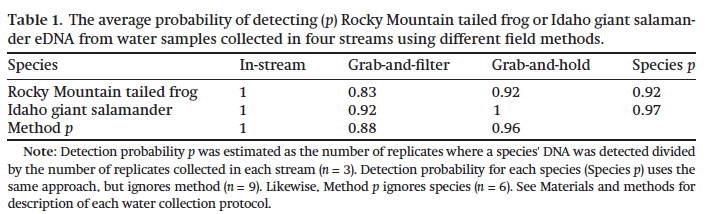
\includegraphics[scale=0.8]{Chapter2Images/rockymountain1.png}
\caption{Comparison of three eDNA sampling methods. Species p refers to the detection probability of the corresponding species \citep{occupancyamphibians}}
\label{fig:comparisonedna}
\end{figure}


Figure~\ref{fig:comparisonedna} illustrates a comparison of three eDNA sampling methods (Goal 2).  In stream methodology had perfect detection, but all three methods produced similar estimates. Note that `Method p' ignores species while `Species p' ignores method and averages over all methods. All three eDNA collection methods produced high detection rates. However, only `In-Stream' filtering led to perfect detection for both species. Researchers did not find any significant difference between any of the three collection methods. 
\vspace{5mm}


To research Goal 1, the researchers  set up standard sampling techniques (using thirty 1m transects randomly placed within 1km upstream of each of the 13 streams where they had taken eDNA samples).  Researchers then counted and weighed all larvae from either species on all the transects. The reason they chose larvae is because this is the most common life stage of the amphibians and thus can be used to infer information regarding adult populations. Larval density and biomass were calculated for each of the 30 transects and the average values were calculated.

\vspace{5mm}

Researchers then performed Backpack electrofishing on the four specified streams 500m upstream from where they had collected eDNA. Researchers then estimated giant salamander density by dividing the number of larvae caught by the total area they searched. Electrofishing allowed the researchers to assure that their methods of kick-net sampling were reliable. Kick-net sampling involves holding a net under the water and kicking the bottom of the substrate in an effort to direct organisms and materials towards and into the net. Indeed, results obtained via electrofishing were excellent predictors of how many larvae had been captured using kick-net sampling (which was done immediately prior to the start of the experiment in each of the four specified streams). (Simple linear regression on eDNA concentration obtained a $R^{2}$ of 0.96 and p-value of p=0.019).


\vspace{5mm}


To investigate the impact of covariates (Goal 3), researchers chose three of the thirteen streams for additional analysis. These were the Deadwood River stream, the East Fork Deadwood stream and the Weir Creek. In the Deadwood river and East Fork, eDNA concentration was measured using the in-stream method for tailed frogs in two reaches 50m apart over a 48-hour period. In Weir Creek, multiple eDNA samples were taken (every 50m for 2km). Following this collection, a three-day multiple removal process (electrofishing) of salamanders took place. The salamanders were removed, weighed and the exact location in which they were removed was recorded. This capture data was used to create a population distribution model for salamanders along the 2km Creek. This data was used to study whether eDNA concentration was impacted by the abundance of salamanders upstream of where the sample was taken.


\vspace{5mm}

For each of the thirteen streams, three replicate samples of surface water were collected. Each sample was taken by pumping 1L of water through a disposable filter funnel with a 47mm diameter cellulose nitrate filter paper. Negative controls were simply 1L of store-bought distilled water. Genetic analysis (qPCR) was then performed on the filter papers. DNA extracted from both species was used to create serial dilutions (standard curves) for comparison. In particular, samples of tissue taken from the tails of each species was used. To quantify the DNA concentration in the
original samples, researchers used a NanoDrop spectrophotometer to estimate the amount of DNA in each sample.

\vspace{5mm}

To compare eDNA concentration estimates obtained from the standard curve among the three different field methods (Goal 4), researchers used a mixed effect model with `stream' as the random effect. Analysis was performed using the SAS software \citep{SAS}. Mixed models are extensions of linear models that allow for the inclusion of both fixed and random effects. 

\vspace{5mm}

Researchers also compared stream-level occupancy and detection probability estimates obtained via standard sampling versus those obtained using eDNA methodology. To test whether eDNA concentration was correlated with abundance, researchers used a General Linear Model. Each of the thirteen streams was a sampling unit and the predictor variables were mean density, mean biomass or proportion of transects occupied (occupancy). The response variable was mean eDNA concentration and was calculated using the three replicate subsamples from each stream (obtained by referring to the standard curve).

\vspace{5mm}

To test for the effect of covariates, further analysis was carried out on the samples obtained from the three specified streams above (Deadwood, East Fork and Weir). Sample location was included as a predictor, along with time of day.

\vspace{5mm}

One main finding of this study was that eDNA detection probabilities does not appear to be influenced by water collection methods. 
In this study, eDNA methodology resulted in better detection rates then simple transect methods.
Finally, in this study, covariates such as time of collection did not appear to be of major impact on calculated eDNA concentration.
In Chapter 5, we consider the impact of environmental covariates on eDNA concentrations in the field.

\newpage

\subsection{eDNA movement}

Because eDNA of aquatic species is shed into streams or rivers, it is crucial that researchers understand how measurement of eDNA is impacted by movement in systems such as complicated, flowing water \citep{ednatransport}. In standing or still waters, measurement of eDNA has been widely used to estimate target species abundance \citep{biomass}. However, studies of eDNA within moving water systems are much less common. In order to study eDNA collected from moving water systems, it is important that researchers understand the biological and physical properties that influence retention and transport of eDNA travelling within these waters.  In Chapter 4, we fit a variety of non-linear models to account for flow and dilution. 

\vspace{5mm}


Researchers have suggested three major mechanisms that impact eDNA  moving systems. Firstly, there is \textit{Transport} (downstream movement driven by bulk water flow),
secondly there is \textit{retention} (deposition or capture by the streambed) and lastly, there is \textit{resuspension} (eDNA embedded in the streambed may become loose or free again) \citep{ednatransport}.

\vspace{5mm}

It has been demonstrated that eDNA in streams is significantly retained by the streambed as it moves down the stream and that concentration of eDNA decreases with downstream distance. Also, although eDNA is deposited on the streambeds, some of this eDNA will end up resuspended in the moving stream \citep{substrate}. More specifically, it has been shown that `fine' substrates such as sand retain more eDNA than `course' substrates such as pea gravel \citep{porous}.



\vspace{5mm}

 \citep{ednatransport}, asked three main questions corresponding to each of the three major mechanisms. 
1), ``How far does an average eDNA particle travel in streams with different hydrologic signatures and how might eDNA detection be used to infer where a species is located?"
2) ``Does surface-subsurface exchange trap eDNA in porous, benthic substrate interstices and does the presence of biofilms of organic matter play a role?"
3) ``Can resuspension from the streambed result in eDNA detection after the source of eDNA has been removed, and how does the characteristic of the streambed impact this?"

\vspace{5mm}


To study these mechanisms, researchers proposed three hypotheses. The first hypothesis was that  downstream transport of eDNA will be limited by hyporheic exchange rates (how quickly water is moving in and out of the stream). In Chapter 4 we  also consider the impact of flow on eDNA movement in a controlled experiment. Figure~\ref{fig:ednatransport} illustrates the three proposed governing mechanisms of eDNA movement in streams.



\begin{figure}[H]
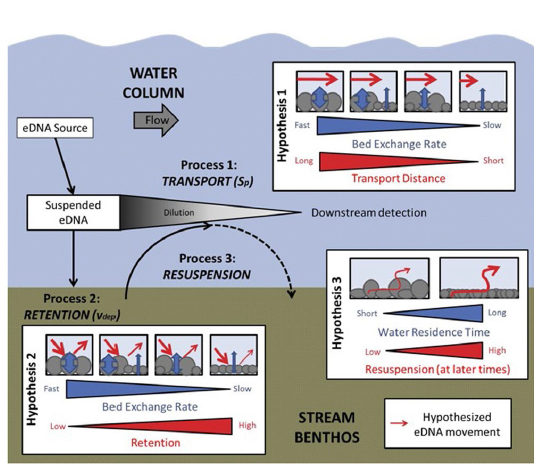
\includegraphics[scale=0.8]{Chapter2Images/ednatransport.png}
\caption{Conceptual diagram depicting the three governing processes of eDNA movement in streams: 1)
Transport, 2) Retention, and 3) Resuspension, and associated hypotheses for eDNA movement \citep{ednatransport}}
\label{fig:ednatransport}
\end{figure}

\vspace{3mm}

Researchers conducted experiments in four streams at the University of Notre Dame Linked Experimental Ecosystem Facility (ND-LEEF) in the summer of 2014. Each of the four streams are 0.4m wide, 7-10cm deep, and 60m long. The water is sourced from a head reservoir fed by groundwater. The four streams are nearly identical in all aspects except that each stream has differing benthic substrate lining the bottom.

\vspace{3mm}

Researchers collected water from a local pond that was known to have a high density of carp. This collected water was then pumped into the head of each of the four streams at a rate of 100mL/min. This was meant to simulate a carp at the head of the stream, whereby it was hypothesized the eDNA would flow or `transport' downstream. The injection of pond water was done for four hours. At the four-hour mark, 15 samples of 250mL were collected at predefined distances from the head of each stream. Once the pump was turned off (simulating fish removal), researchers continued to collect samples at regular timed intervals. The samples were stored and transferred to the lab, where qPCR was performed.

\vspace{3mm}

 To quantify the number of DNA copies in each extract, researchers created a synthetic standard curve and included it on each qPCR plate along with the DNA extracts. Since researchers knew the amount of DNA in their dilution series, they were able to create a standard curve for carp concentration. By comparing the known molecular weights with the obtained CT scores, the researchers were able to apply linear regression to create the standard curve. Moreover, the researchers were able to estimate the number of DNA copies in samples by dividing the estimated molecular weight of the DNA by Avogadro’s number. The LoD used in this study was 30 copies of DNA per reaction. The LoD was chosen based on the creation of the standard curve, as 30 copies of DNA per reaction resulted in a detection in 95\% of reactions.


\begin{figure}[H]
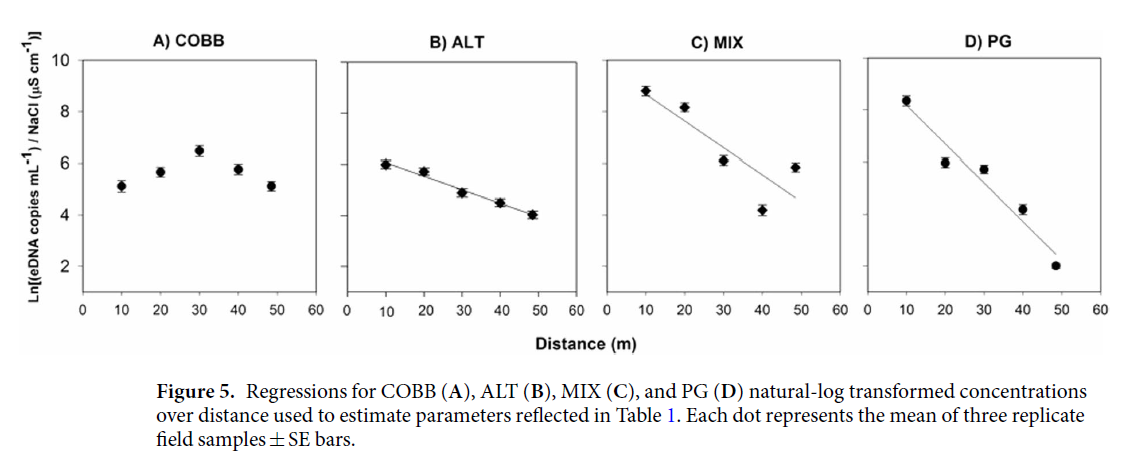
\includegraphics[scale=0.6]{Chapter2Images/transport2.png}
\caption{Results of the flow experiment \citep{ednatransport}. Stream PG has a smooth substrate, while COBB has course substrate. ALT and MIX have substrates in between course and smooth.}
\label{fig:ednatransport2}
\end{figure}

In general, eDNA concentration decreased as the distance from the head of the streams increased (Figure~\ref{fig:ednatransport2}). However, differences in substrate also resulted in different concentrations down the streams. COBB, ALT, MIX and PG are codes for each of the four streams. COBB has a more course substrate, while ALT and MIX have intermediate substrates. PG has a smooth substrate. NaCl was added to the mixture to help stabilize the DNA. The points plotted are the log transformed mean number of estimated copy numbers from each set of replicates, with the associated line of best fit created using simple linear regression.

\newpage



\subsection{Temperature}

Water temperature is known to be highly influential to the metabolism of fish \citep{tempmet}. The exact impact that temperature has on eDNA release is still not completely understood. It has been shown that in general, higher water temperature does increase the metabolism of fish (which may result in more DNA being shed).

\vspace{5mm}

 One study \citep{fishabundance} researched the question of how water temperature and the eDNA capture method impact the relationship between eDNA concentration and fish abundance. Researchers collected Brook Charr fingerlings from a fish hatchery in Cap-Sante, Quebec.  The fish were stored and returned alive to the lab. Fifteen tanks were prepared with water at $\ang{7}$ C, and another fifteen tanks were prepared with water $\ang{14}$ C.


\begin{figure}[H]
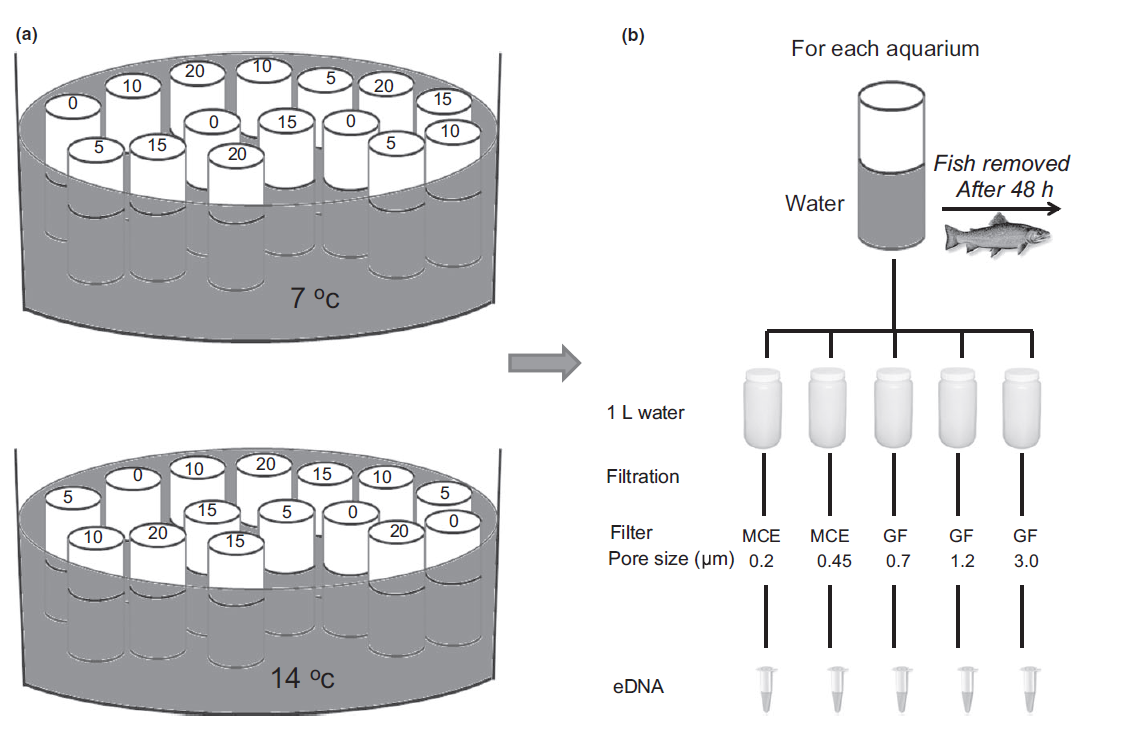
\includegraphics[scale=0.5]{Chapter2Images/brookchar.png}
\caption{Experimental design of Brook Charr exposed to $\ang{7 }$ C and $\ang{14}$C and (b) eDNA collection procedures  \citep{fishabundance}. Fish abundance for each
water temperature was randomly assigned. eDNA was captured via filtration (MCE, mixed cellulose ester filters; GF, glass fiber).}
\label{fig:brookchar}
\end{figure}

\newpage

For each of the two distinct temperatures, 0, 5, 10, 15 and 20, Brook Charr were placed into the 30 tanks (Figure~\ref{fig:brookchar}). For each temperature, each abundance of fish was repeated three times. That is, three tanks at $\ang{7}$ C contained 5 fish and three tanks at $\ang{14}$ C also contained 5 fish. The same was done for each number of fish. The zero fish triplicates represent negative controls, i.e. an abundance of 0.

\vspace{5mm}

The total biomass of fish in each tank was measured by comparing the weight of the tanks prior to the addition of the fish to the weight after they were added. The fish were then given five days to live in each tank. Each tank was then removed and let to sit in the dark for 48 hours, at which point the fish were removed. Once removed, the water in each 1L triplicate was mixed and then filtered using various filters and pore sizes to collect eDNA. DNA was extracted using the salt extraction method. A 139-basepair unique to Brook Charr was used as the target DNA. A standard curve was created using known 7 known dilutions of Brook Charr eDNA. eDNA concentration of samples was then quantified using real-time Taq-Man PCR and comparison to the 7-point standard curve previously created.


\vspace{5mm}

A Mann-Whitney test was used to test for significance in the mean eDNA concentration between the two separate temperatures (there were 150 fish for both temperatures for a total of 300 fish).
A Cook’s distance test was used to detect potential outliers and influential points. At all levels of fish abundance, higher eDNA levels (more concentrated) were found in the $\ang{14}$ C samples compared to the $\ang{7}$ C samples when using glass fiber (GF) filters. For a few filters that are known to have a low level of eDNA collection, such as MCE(2 $\mu L$), differences in eDNA at the two temperatures were not detected.

\vspace{5mm}
The results of this experiment showed that the concentration of eDNA  did increase significantly at higher temperatures. Researchers hypothesized this may be due to the fact that fish mobility is increased at higher temperatures \citep{fishmobility}, moreover at higher temperature the rate at which skin cells are shed and other secretions are released is increased.  Hence, temperature may need to be considered when a data analysis on eDNA on aquatic species is performed. This is particularly important when using fine filters that are known to capture high levels of eDNA. In Chapter 5, we consider the possible impact of temperature on eDNA concentrations as well.